\documentclass{beamer}
\setbeamersize{text margin left=3mm,text margin right=3mm}

\usepackage[backend=bibtex, natbib=true, style=authoryear]{biblatex}% \usepackage[style=authoryear]{natbib}
% \bibliographystyle{plain}
\addbibresource{bibliography}

\usepackage{amsmath, bm, amssymb}
\usepackage{tcolorbox}
\usepackage{graphicx}
\usepackage{xcolor}
\usepackage{listings}
%New colors defined below
\definecolor{codegreen}{rgb}{0,0.6,0}
\definecolor{codegray}{rgb}{0.5,0.5,0.5}
\definecolor{codepurple}{rgb}{0.58,0,0.82}
\definecolor{backcolour}{rgb}{0.95,0.95,0.92}

%Code listing style named "mystyle"
\lstdefinestyle{mystyle}{
  backgroundcolor=\color{backcolour}, commentstyle=\color{codegreen},
  keywordstyle=\color{magenta},
  numberstyle=\tiny\color{codegray},
  stringstyle=\color{codepurple},
  basicstyle=\ttfamily\footnotesize,
  breakatwhitespace=false,
  breaklines=true,
  captionpos=b,
  keepspaces=true,
  numbers=left,
  numbersep=5pt,
  showspaces=false,
  showstringspaces=false,
  showtabs=false,
  tabsize=2
}
\lstset{style=mystyle}


\usepackage{hyperref}
\hypersetup{
    colorlinks=true,
    linkcolor=blue,
    filecolor=magenta,
    urlcolor=cyan,
    pdftitle={Overleaf Example},
    pdfpagemode=FullScreen,
    }
\usepackage{multirow}
\usetheme{Boadilla}
\usecolortheme{seahorse}
\newcommand{\thetab}{\boldsymbol{\theta}}
\newcommand{\xb}{\boldsymbol{x}}
\newcommand{\red}[1]{\textcolor{red}{#1}}
\newcommand{\blue}[1]{\textcolor{blue}{#1}}

\DeclareMathOperator*{\argmin}{arg\,min}
\DeclareMathOperator*{\argmax}{arg\,max}

\title[RegionalRHALE - TaDA @ VLDB 2024]{Fast and accurate regional effect plots for automated tabular
data analysis}
\subtitle{TaDA Workshop @ VLDB 2024}
\author[Gkolemis, Vasilis] % (optional)
{Vasilis Gkolemis\inst{1,2} \and
  Christos Diou\inst{2} \and
  Eirini Ntoutsi\inst{3} \and
  Theodore Dalamagas\inst{1}
}

\institute[ATH-HUA]{
  \inst{1} ATHENA Research and Innovation Center
  \and %
  \inst{2} Harokopio University of Athens
  \and
  \inst{3} University of the Bundeswehr Munich
}

\date{August 2024}


% Use a simple TikZ graphic to show where the logo is positioned
% \logo{\begin{tikzpicture}
% \filldraw[color=red!50, fill=red!25, very thick](0,0) circle (0.5);
% \node[draw,color=white] at (0,0) {LOGO HERE};
% \end{tikzpicture}}

%End of title page configuration block
%------------------------------------------------------------
%The next block of commands puts the table of contents at the
%beginning of each section and highlights the current section:

\AtBeginSection[]
{
  \begin{frame}
    \frametitle{Program}
    \tableofcontents[currentsection]
  \end{frame}
}


% ------------------------------------------------------------
\begin{document}
\frame{\titlepage}
%---------------------------------------------------------


\section{ML + XAI $\rightarrow$ a good Data Analysis Pipeline (5')}

\begin{frame}
  \frametitle{Problem Statement}
  \begin{figure}[ht]
    \centering
    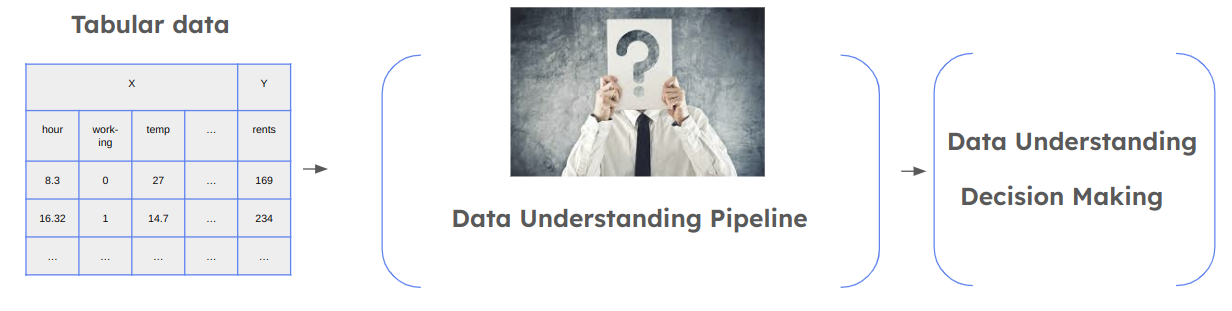
\includegraphics[width=\textwidth]{./figures/problem_statement.png}
  \end{figure}
\end{frame}

\begin{frame}
  \frametitle{Idea 1}
  \begin{figure}[ht]
    \centering
    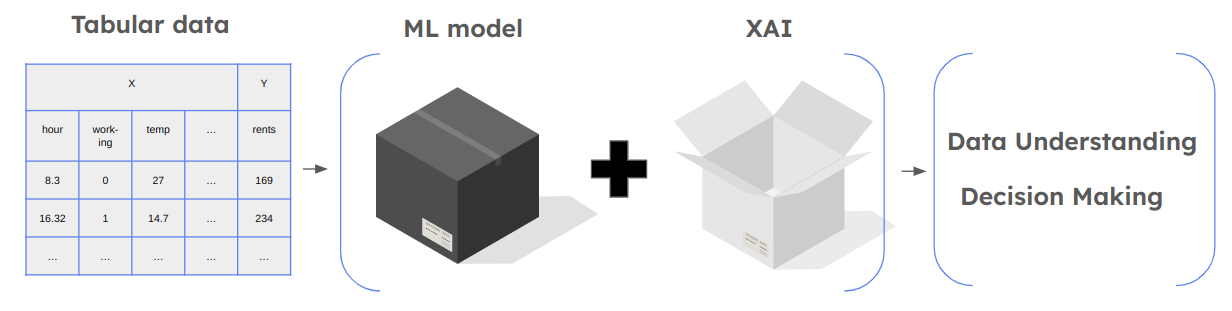
\includegraphics[width=\textwidth]{./figures/convincing_point_1.png}
  \end{figure}
  \noindent\makebox[\linewidth]{\rule{\paperwidth}{0.4pt}}
  Black box ML model + XAI = a Data Analysis pipeline!
\end{frame}

\begin{frame}
  \frametitle{Idea 2}
  \begin{figure}[ht]
    \centering
    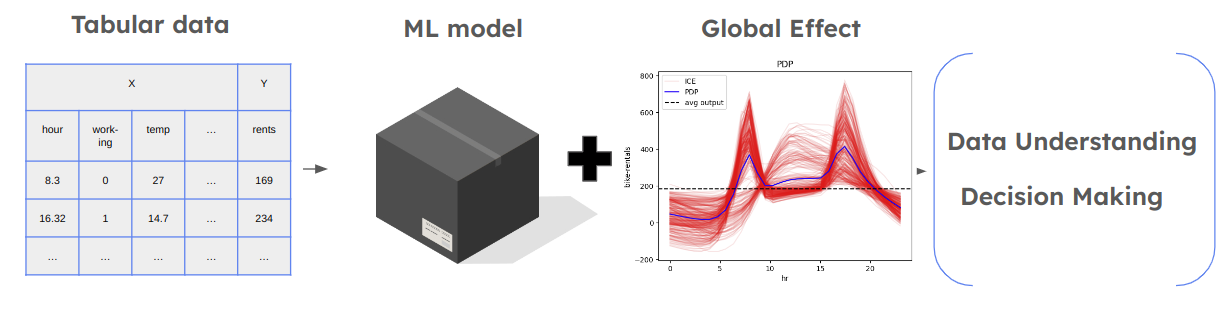
\includegraphics[width=\textwidth]{./figures/convincing_point_2.png}
  \end{figure}
  \noindent\makebox[\linewidth]{\rule{\paperwidth}{0.4pt}}
  Global effects is a good XAI choice!
\end{frame}

\begin{frame}
  \frametitle{Idea 3}
  \begin{figure}[ht]
    \centering
    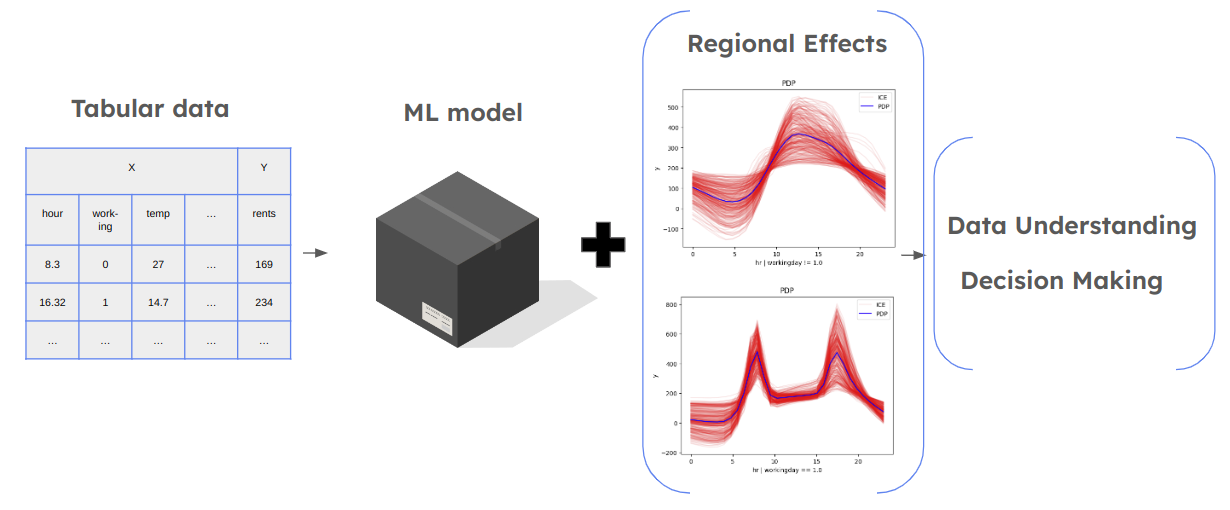
\includegraphics[width=\textwidth]{./figures/convincing_point_3.png}
  \end{figure}
  \noindent\makebox[\linewidth]{\rule{\paperwidth}{0.4pt}}
  Regional effects is a better XAI choice!
\end{frame}

\begin{frame}
  \frametitle{Idea 4}
  \begin{figure}[ht]
    \centering
    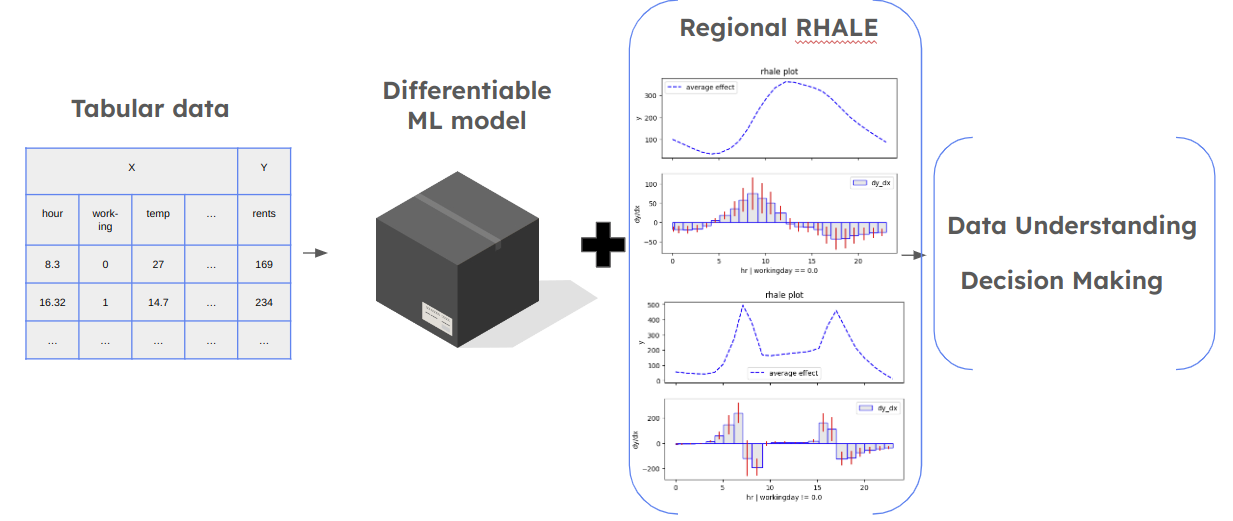
\includegraphics[width=\textwidth]{./figures/convincing_point_4.png}
  \end{figure}
  \noindent\makebox[\linewidth]{\rule{\paperwidth}{0.4pt}}
  Use RegionalRHALE if the black box model is differentiable!
\end{frame}

% \begin{frame}
%   \frametitle{Feature Effect}
%   \begin{itemize}
%     \item $f(\cdot): \mathbf{x} \rightarrow y \longrightarrow f_i(\cdot): x_i \rightarrow y \: \forall i $
%   \end{itemize}
%   \vspace{2mm}
%   \begin{figure}[ht]
%     \centering
%     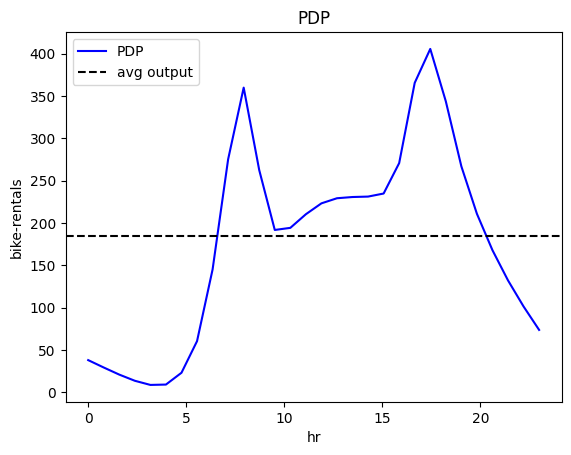
\includegraphics[width=0.5\textwidth]{./figures/bike_sharing_global_pdp.png}
%   \end{figure}

%   \noindent\makebox[\linewidth]{\rule{\paperwidth}{0.4pt}}
%   Simple and intuitive.
% \end{frame}

% \section{Feature Effect}
% \subsection{Bike-sharing dataset}

\begin{frame}
  \frametitle{Bike-sharing dataset}
  \begin{itemize}
  \item hourly count of bike-rentals (2011, 2012)
  \item Design-matrix $X$:
    \begin{itemize}
    \item year, month, day, \red{hour}
    \item working day vs. non-working day
    \item temperature
    \item humidity
    \item windspeed
    \end{itemize}
  \item Target variable $Y$:
    \begin{itemize}
    \item bike-rentals per hour
      \begin{itemize}
      \item $Y_\mu = 189.5$
      \item $Y_\sigma = 181.4$
      \end{itemize}
    \end{itemize}
  \item Decision Making: \red{decide a discount policy}
  \item Data Understanding: how bike rental market works
  \end{itemize}
\end{frame}


\begin{frame}
  \frametitle{Proposed pipeline: Fit and Explain}
  \begin{itemize}
  \item \red{decide a discount policy}
    \begin{itemize}
    \item which hour of the day to apply the discount
    \item how the feature $x_{\mathtt{hour}}$ relates to $y_{\mathtt{bike\_rentals}}$
    \end{itemize}

  \item Step 1: Fit a black-box ML model
    \begin{itemize}
    \item Could be any ML model
    \item a Neural Network achieves $\texttt{RMSE} \approx 45.35 $ counts ($0.25Y_\sigma$)
    \end{itemize}
  \item Step 2: Use feature effect
    \begin{itemize}
    \item Global effect: $x_{\mathtt{hour}}$ vs $y_{\mathtt{bike\_rentals}}$ globally
    \item Regional effect: $x_{\mathtt{hour}}$ vs $y_{\mathtt{bike\_rentals}}$ regionally
    \end{itemize}
  \end{itemize}

  \noindent\makebox[\linewidth]{\rule{\paperwidth}{0.4pt}}
  Let's see!
\end{frame}

\begin{frame}
  \frametitle{Global Effect: PDP and RHALE}
  \begin{figure}[ht]
    \centering
    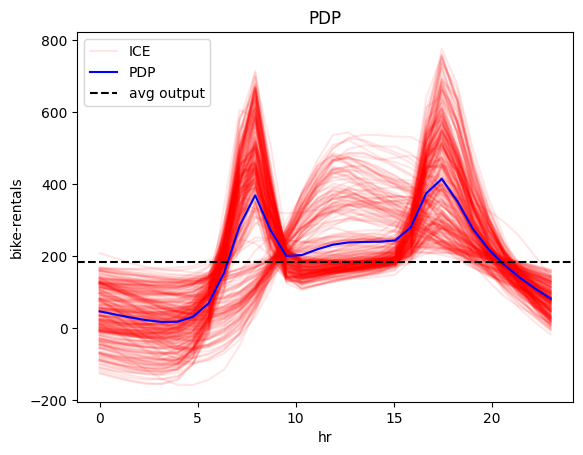
\includegraphics[width=0.45\textwidth]{./figures/bike_sharing_global_pdp_heterogeneity.png}
    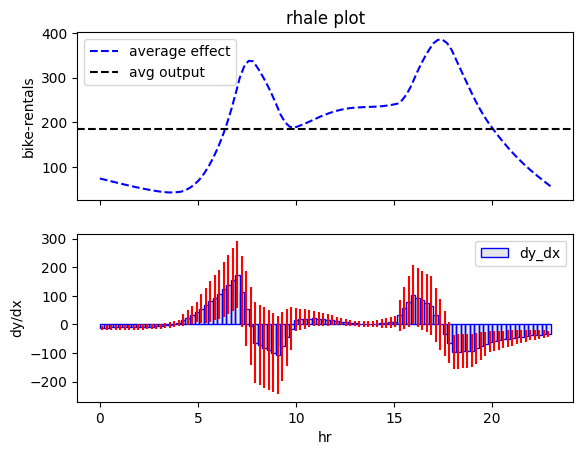
\includegraphics[width=0.45\textwidth]{./figures/bike_sharing_global_rhale_heterogeneity.png}
  \end{figure}
  \noindent\makebox[\linewidth]{\rule{\paperwidth}{0.4pt}}
  PDP and RHALE~\citep{gkolemis2023rhale} are global effect methods
\end{frame}

\begin{frame}
  \frametitle{Regional Effect: Regional-PDP}
  \begin{figure}[ht]
    \centering
    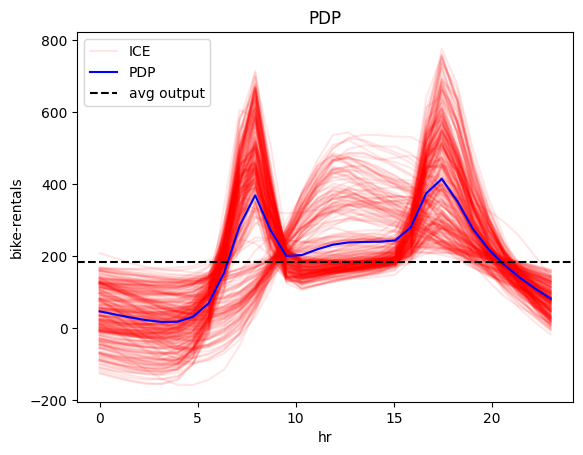
\includegraphics[width=0.33\textwidth]{./figures/bike_sharing_global_pdp_heterogeneity.png}\\
    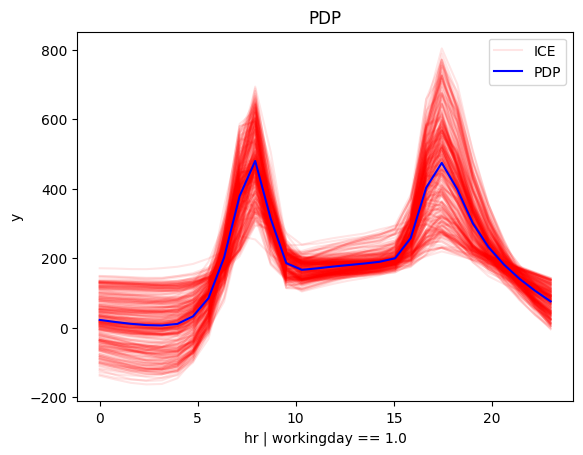
\includegraphics[width=0.33\textwidth]{./figures/bike_sharing_regional_pdp_workingdays.png}
    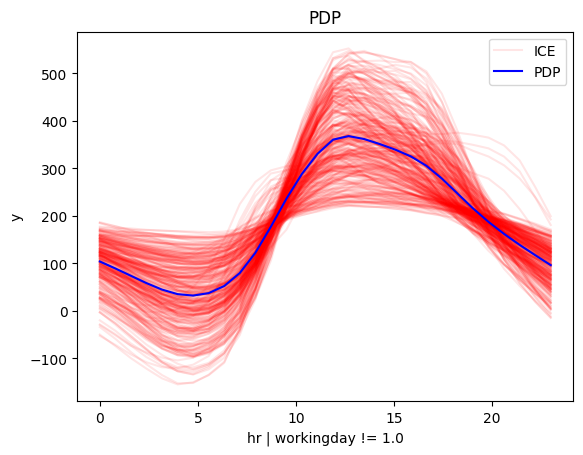
\includegraphics[width=0.33\textwidth]{./figures/bike_sharing_regional_pdp_weekends.png}
  \end{figure}
  \noindent\makebox[\linewidth]{\rule{\paperwidth}{0.4pt}}
  Regional PDP~\citep{herbinger_repid_2022}
\end{frame}

\begin{frame}
  \frametitle{Regional Effect: Regional-RHALE}
  \begin{figure}[ht]
    \centering
    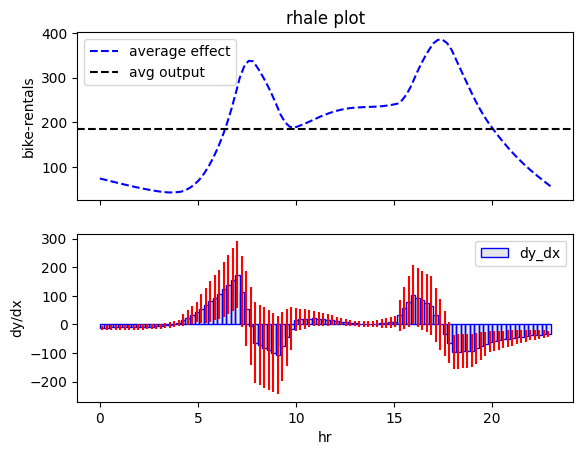
\includegraphics[width=0.33\textwidth]{./figures/bike_sharing_global_rhale_heterogeneity.png} \\
    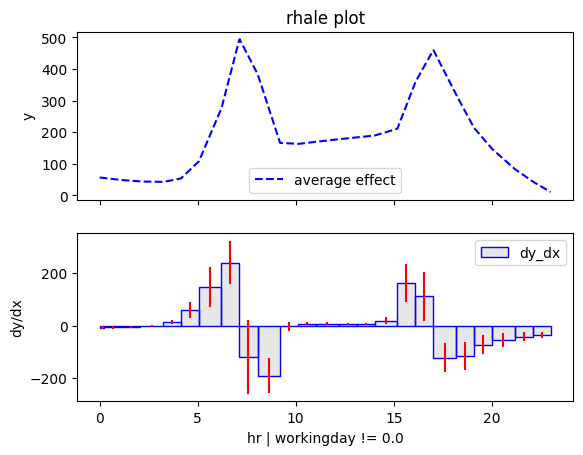
\includegraphics[width=0.33\textwidth]{./figures/bike_sharing_regional_rhale_workingdays.png}
    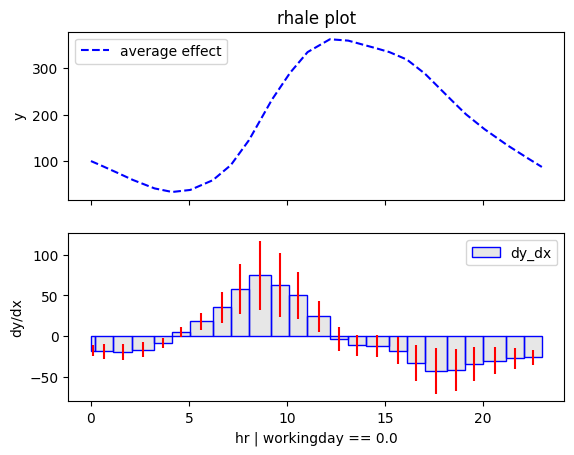
\includegraphics[width=0.33\textwidth]{./figures/bike_sharing_regional_rhale_weekends.png}
  \end{figure}
  \noindent\makebox[\linewidth]{\rule{\paperwidth}{0.4pt}}
  Regional RHALE - our proposal!
\end{frame}

\section{RegionalRHALE: a good XAI choice (4')}

\begin{frame}
  \frametitle{RegionalRHALE - How it works (a)}
  \begin{itemize}
  \item RHALE plot~\citep{gkolemis2023rhale}
  \item red bars express the heterogeneity
  \end{itemize}
  \begin{figure}[ht]
    \centering
    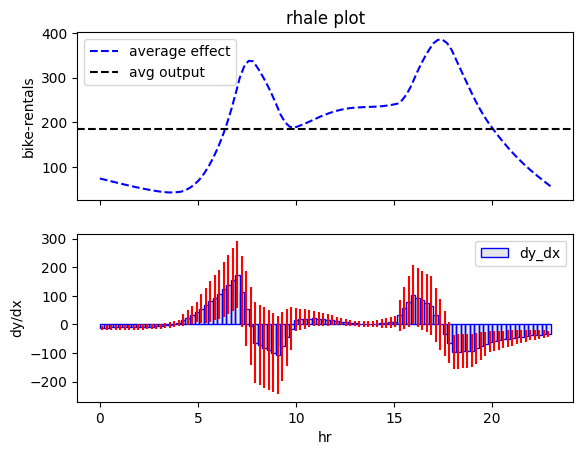
\includegraphics[width=0.6\textwidth]{./figures/bike_sharing_global_rhale_heterogeneity.png}
  \end{figure}
\end{frame}

\begin{frame}
  \frametitle{Regional RHALE - How it works (b)}
  \begin{itemize}
  \item iterate over all other features
  \item select the split with the maximum heterogeneity reduction
  \end{itemize}
  \begin{figure}[ht]
    \centering
    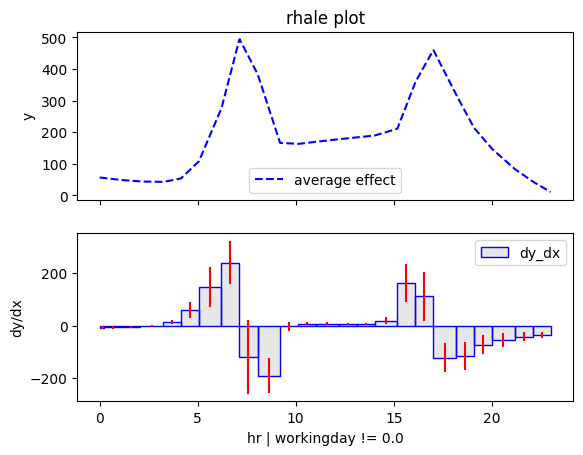
\includegraphics[width=0.49\textwidth]{./figures/bike_sharing_regional_rhale_workingdays.png}
    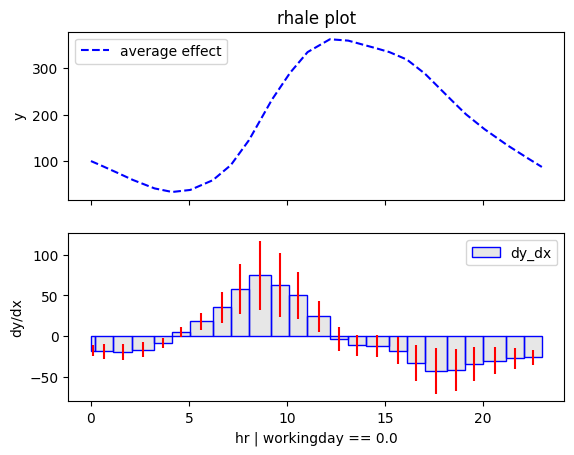
\includegraphics[width=0.49\textwidth]{./figures/bike_sharing_regional_rhale_weekends.png}
  \end{figure}
\end{frame}


\begin{frame}
  \frametitle{Regional RHALE is fast}
  \begin{itemize}
  \item iterating over all other features $\rightarrow$ is slow
  \item needs fast evaluation of the heterogeneity
  \item if model is differentiable, regional RHALE is very fast
  \item regional RHALE treats well cases with correlated features
  \end{itemize}
  \begin{figure}[ht]
    \centering
    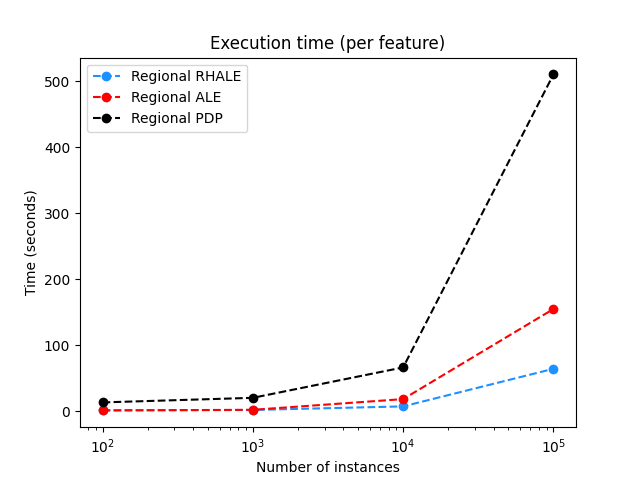
\includegraphics[width=0.45\textwidth]{./figures/simulation_2/efficiency_samples.png}
    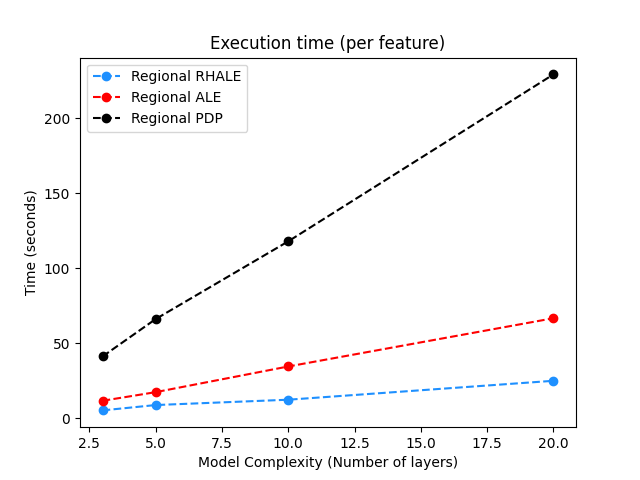
\includegraphics[width=0.45\textwidth]{./figures/simulation_2/efficiency_layers.png}
  \end{figure}
\end{frame}

\section{\texttt{Effector} - a \texttt{Python} Package for Feature Effect (1')}

\begin{frame}
  \frametitle{\texitt{Effector} - a \textt{Python} package for feature effect}
  \begin{itemize}
  \item Implements:
    \begin{itemize}
    \item many global effect methods (PDP, RHALE, SHAP-DP)
    \item many regional effect methods (regionalPDP, regionalRHALE, regionalSHAP-DP)
    \end{itemize}
  \item Work in progress
  \item If you are interested, please use it and give feedback
  \item Source: \href{https://github.com/givasile/effector}{https://github.com/givasile/effector}
  \item Documentation: \href{https://xai-effector.github.io/}{https://xai-effector.github.io/}
    \end{itemize}
\end{frame}


\begin{frame}[allowframebreaks]
  \frametitle{References}
  \printbibliography
\end{frame}

\end{document}
